\NeedsTeXFormat{LaTeX2e}
\documentclass[11pt]{article}
\usepackage{url}
\usepackage{amsmath}
\usepackage{amsthm}
\usepackage{amssymb}
\usepackage{mathpartir}
\usepackage{graphicx}
\usepackage{comment}


\newcommand{\deftech}[1]{\textbf{#1}}
\newcommand\mrel{\mathop{\mathbf{r}}}
\newcommand\morel{\mathop{\mathbf{r}'}}
\newcommand\menv{\rho}
\newcommand\mval{v}
\newcommand\mans{a}
\newcommand\mint{i}
\newcommand\moint{j}
\newcommand\mbool{b}

\newcommand\plug[2]{#1[#2]}

\newcommand\merr{r}

\newcommand\mctx{\mathcal{C}}
\newcommand\mectx{\mathcal{E}}
\newtheorem{theorem}{Theorem}
\newcommand\Err{\mathit{Err}}
\newcommand\Plus{\mathit{Plus}}
\newcommand\Mult{\mathit{Mult}}
\newcommand\Succ{\mathit{Succ}}
\newcommand\Pred{\mathit{Pred}}
\newcommand\Eq{\mathit{Eq}}
\newcommand\True{\mathit{True}}
\newcommand\False{\mathit{False}}
\newcommand\If{\mathit{If}}
\newcommand\Div{\mathit{Div}}

\newcommand\reduce{\mathop{\mathbf{b}}}

\newcommand\areducename{\mathbf{a}}
\newcommand\areduce[2]{#1\;\areducename\;#2}

\newcommand\step{\rightarrow_\mathbf{b}}
\newcommand\multistep{\rightarrow^\star_\mathbf{b}}

\newcommand\astdstep{\longmapsto_{\reduce}}
\newcommand\astdmultistep{\longmapsto^\star_{\reduce}}

\newcommand\breducename{\mathbf{b}}
\newcommand\errreducename{\mathbf{err}}
\newcommand\propreducename{\mathbf{prop}}
\newcommand\bvreducename{\mathbf{bv}}
\newcommand\bstepname{\rightarrow_{\breducename}}
\newcommand\bmultistepname{\rightarrow^\star_{\breducename}}

\newcommand\bmultistep[3]{#1\vdash #2\;\bmultistepname\;#3}
\newcommand\bstdstep[3]{#1\vdash #2\;{\longmapsto_{\breducename}}\;#3}
\newcommand\bstdmultistep[3]{#1\vdash #2\;{\longmapsto^\star_{\breducename}}\;#3}

\newcommand\breduce[3]{#1 \vdash {#2}\;\breducename\; {#3}}
\newcommand\errreduce[3]{#1 \vdash {#2}\;\errreducename\; {#3}}
\newcommand\propreduce[3]{#1 \vdash {#2}\;\propreducename\; {#3}}
\newcommand\bvreduce[3]{#1 \vdash {#2}\;\bvreducename\; {#3}}
\newcommand\bstep[3]{#1 \vdash {#2}\;\rightarrow_{\breducename}\; {#3}}
\newcommand\bclosedstep[2]{{#1}\;\rightarrow_{\breducename}\; {#2}}

\newcommand\laxparstep{\rightrightarrows_\mathbf{a}}
\newcommand\maxparstep{\rightrightarrows'_\mathbf{a}}


\newcommand{\xdown}[1]{X_{#1 \downarrow}}
\newcommand{\xup}[1]{X_{#1 \uparrow}}
\newcommand{\xdownk}[2]{X_{#1 \downarrow #2}}
\newcommand{\xupk}[2]{X_{#1 \uparrow #2}}
\newcommand{\xblock}[1]{[x_{#1 1}, x_{#1 2} , \dots, x_{#1 \frac{1}{c}}]^{\top}}
\newcommand{\conpr}[2]{Pr[#1\,|\,#2]}
\newcommand{\priv}{{\bf priv}(X)}
\newcommand{\alt}[1]{{\bf alt}(X_{#1})}
\newcommand{\xbot}[1]{x_{#1 \frac{1}{c}}}
\newcommand{\cwp}[1]{(\epsilon, \delta, \Delta_{#1}, \Gamma)}


\newcommand\Arith{\mathcal{A}}
\newcommand\Barith{\mathcal{B}}

\newcommand\Var{\mathit{Var}}

\newcommand{\mvar}{x}
\newcommand\s[1]{\mathit{#1}}

\title{Composition Theorem for streaming CW-pricacy}
\date{}
\begin{document}
\maketitle

\section{Characterize Privacy as Regions}
In this section, we show how to characterize Differential Privacy (DP) and CW-Privacy (CW-P) in terms of convex regions, and how to compute the $(\epsilon, \delta)$ values for each mechanism in terms of tangent lines of such convex regions. We focus on the context of finite discrete states for the simplicity of analysis.
\subsection{Case of DP}
Let ${\cal X} $ be the set of all databases. Let ${\cal Y}$ be the set of all out comes of mechanism $M$. $M$ is a probability measure from $\cal X$ to $\cal Y$. For simplicity of analysis, assume $|{\cal X}| =n $ and $|{\cal Y}|=m$. Then, $M$ corresponds to an $n \times m$ Markov matrix ${M} =[M(x_{1}), \dots , M(x_{n})]^{\top}$.


Now, it is easy to see the following is an equivalent definition of DP.
\begin{theorem}
For any $\epsilon \geq 0$ and $\delta \in [0, 1]$, a mechanism $M$ is $(\epsilon, \delta)$-differentially private if and only if the following conditions are satisfied for all pairs of neighboring databases $x$ and $x'$, and all region $S \subseteq {\cal Y}$:
\[
Pr[M(x) \in S]+e^{\epsilon}Pr[M(x') \in \bar{S}] \geq 1-\delta , \quad and
\]
\[
e^{\epsilon}Pr[M(x) \in S]+Pr[M(x') \in \bar{S}]  \geq 1-\delta .
\]
\end{theorem}
This gives a graphical representation (region) of DP:
\[
R(\epsilon, \delta) = \{(p_{x},p_{y}) \,|\, p_{x}+e^{\epsilon}p_{y} \geq1 - \delta,  e^{\epsilon}p_{x}+p_{y} \geq 1 - \delta\} .
\]
For any two databases $x$ and $x'$, define
\[
R(M, x, x') = convex \{(Pr[M(x) \in S], Pr[M(x') \in \bar{S}]) \,|\, \text{for all }S \subseteq {\cal Y} \}
\]
$R(M,x,x')$ has the following equivalent form.
\[
R(M,x,x') = \{ (M(x) \cdot {\bf \alpha}, M(x') \cdot {\bf \beta}) \,|\, 0 \leq \alpha_{i}, \beta_{i} \leq 1, \, {\bf \alpha} +{\bf \beta} = {\bf 1^{m}} \},
\] 
where $\cdot$ denote the dot production of vectors.
\begin{definition}
For any mechanism $M$, we define its privacy region $R(M) = \bigcup_{(x , x')} R(M, x, x') $, where $(x,x')$ is a pair of neighboring databases.
\end{definition}
Immediately, it should not hard to see the following theorem.
\begin{theorem}
 $M$ is $(\epsilon, \delta)$-differentially private iff $R(M) \subseteq R(\epsilon, \delta) $.
 \end{theorem}
\begin{figure}[th]
\centering
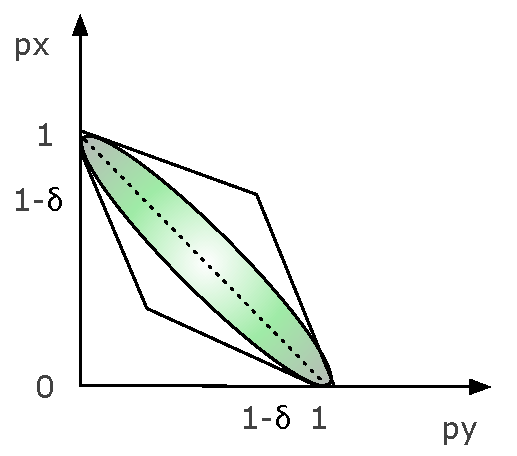
\includegraphics[width=2.5in]{fig/privacyregion.pdf}
\caption{\label{privacy_region} Every tangent line of the privacy region forms a pair of $(\epsilon, \delta)$. }
\end{figure}
As it is shown in Figure~\ref{privacy_region}, every tangent line of the privacy region corresponds to a pair of $(\epsilon, \delta)$. In general, the privacy region $R(M, x, x')$ of any mechanism $M$ can be represented by the intersections of all such regions $\{R(\epsilon_{i}, \delta_{i})\}$, which is completely described by the set of slopes and shifts $\{(\epsilon_{i}, \delta_{i})\}$.
\begin{enumerate}
\item For the set slopes, let ${\cal E} = \{0 \leq \epsilon_{i} < \infty \,|\, Pr[M(x)=y] = e^{\epsilon_{i}}Pr[M(x')=y] \text{ for some $y \in {\cal Y}$} \}$
\item For each $\epsilon_{i}$,  $\delta_{i} = \max_{S \subseteq {\cal Y}} \{ \Sigma_{y \in S}Pr[M(x)=y] - e^{\epsilon_{i}}\Sigma_{y \in S}Pr[M(x)=y]\}$
\end{enumerate}
\subsection{Case of CW-P}
In the case of CW-P, we use $X$ to denote a database variable that follows some distribution $D$. Let the pmf of $D$ be $f_{D} =[{f_{x_{1}} , \dots, f_{x_{n}}}]$. Let $alt(X)$ denote a scrubbed version of $X$. Assume $alt(X)$ follows some distribution $D'$ with pmf $f'_{D}$.

It is easy to see that CW-P has the following equivalent definition.
\begin{theorem}
For any $\epsilon \geq 0$ and $\delta \in [0, 1]$, a mechanism $M$ is $(\epsilon, \delta)$-differentially private if and only if the following conditions are satisfied for all distributions on $D$ on $(X, Z)$, all $(priv, alt)$ pairs, and all region $S \subseteq {\cal Y}$:
\[
Pr[M(X) \in S \,|\, priv(X), Z]+e^{\epsilon}Pr[M(alt(X)) \in \bar{S}\,|\, priv(X), Z] \geq 1-\delta , \quad and
\]
\[
e^{\epsilon}Pr[M(X) \in S\,|\, priv(X), Z]+Pr[M(alt(X)) \in \bar{S}\,|\, priv(X), Z]  \geq 1-\delta ,
\]
where $M(X) = f_{D}M$ and $M(alt(X))=f'_{D}M$.
\end{theorem}
Notice mechanism $M' = [f_{D}M, f'_{D}M]^{\top}$ can be seen as a DP version of $M$. Hence, CW-P also has form of privacy regions, and everything else described above follows.
\section{Composition Theorem of CW-P in the streaming setting}


\end{document}
